\chapter{Implementation}
% This chapter may be called something else\ldots but in general the
% idea is that you have one (or a few) ``meat'' chapters which describe
% the work you did in technical detail.
\begin{tcolorbox}[boxsep=0mm,left=2.5mm,right=2.5mm]
    \textbf{Design and Implementation:} {\em In this section, I will outline the
    goals of my system. I will give a brief overview of the chapter structure,
    summarising each core section and what I achieve.}
\end{tcolorbox}

\section{System Architecture}
\label{sec:sys-arch}
\begin{figure}[h]
    \centering
    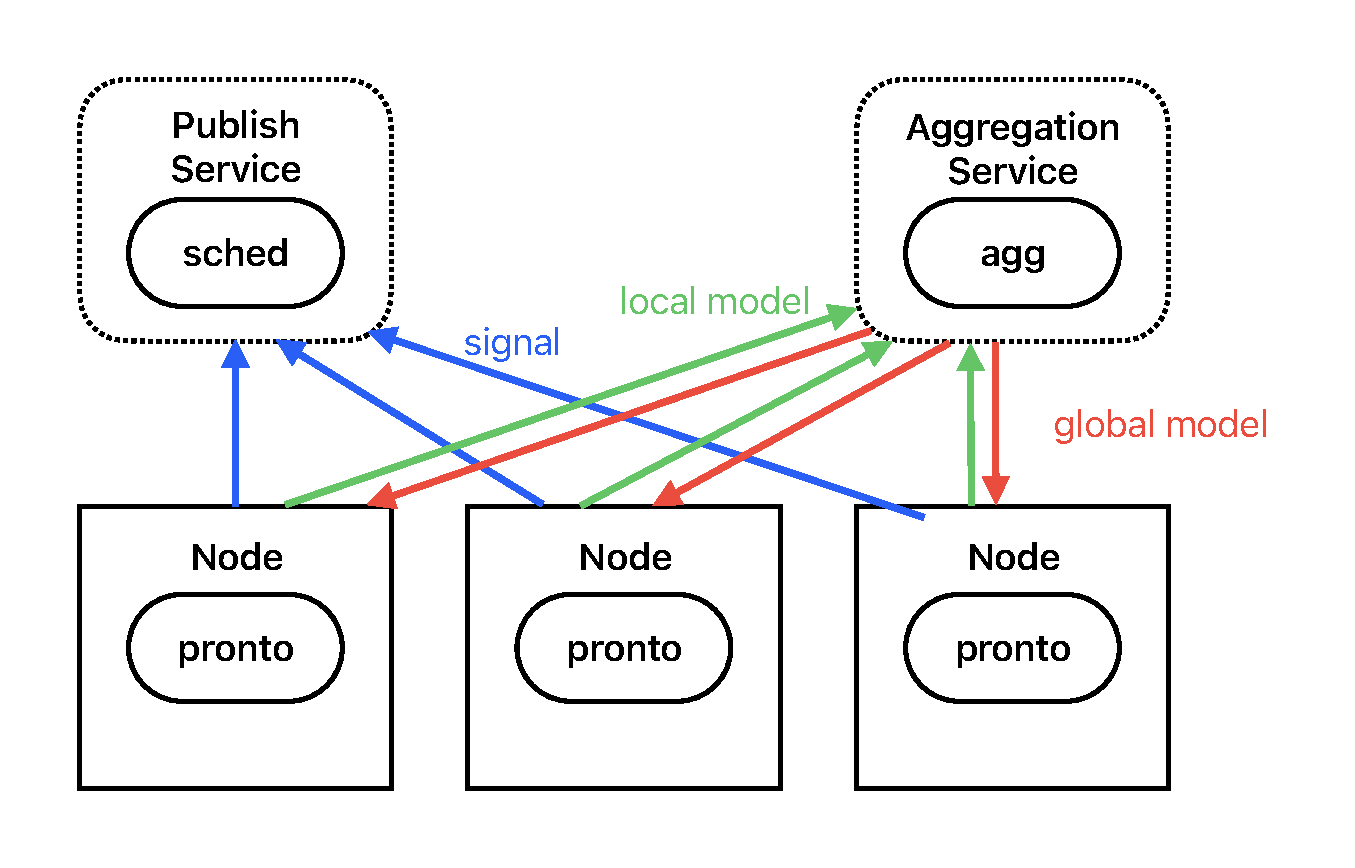
\includegraphics[width=\textwidth]{images/system.pdf}
    \caption{The components within the Pronto system}
    \label{pronto-system}
\end{figure}

The Pronto system consists of three core components (shown in figure
\ref{pronto-system}):
\begin{itemize}
    \item Pronto DaemonSet: each node in the cluster will have a pronto pod
        running on it. This pod collects telemetry of the node performance and
        generates its local model and a willingness signal. When the Pronto pod
        deems its local model outdated, it requests the latest aggregated global
        model from the Aggregation service. In addition, it periodically
        generates and publishes its willingness signal to the Publish service.
    \item Scheduler: In Pronto, the scheduler is a \textbf{Scheduler Plugin}, implementing custom
        Filter, Score and Reserve functions. It also acts as the server of the
        Publish service, collecting the latest willingness scores of each node
        which it uses in its scheduling decisions.
    \item Aggregator: This deployment provides the Aggregation service. The
        underlying \verb|pronto-agg| pod receives local models from nodes and
        returns the latest aggregated global model.
\end{itemize}

\section{Applying Pronto For Kubernetes}

\subsection{Metric Selection}
In the paper, Pronto uses \verb|CPU-Reeady| which is generated by the VMware
vSphere virtualisation platform. This metric can't be used within a
Kubernetes cluster as machines can be both virtual and physical. Since Linux
4.20+, the kernel can track how long tasks are stalled waiting for the CPU
at a cgroup granularity. By inspecting the the root cgroup’s CPU pressure
file using \verb|cat /proc/pressure/cpu| you can measure the total time all
processes spent waiting for the CPU to be available.

While this type of metric can be used to alert of performance degradation,
this metric has a few shortcomings. Firstly, it only reports CPU-centric
information. This is not always representative measure of resource
contention as memory-heavy workloads may starve for RAM resources while
metrics like \verb|CPU-Ready| and \verb|/proc/pressure/cpu| remain
unaffected.
\begin{figure}[h]
    \centering
    
\includegraphics[width=\textwidth]{images/blank.pdf}
    \caption{The values of \texttt{/proc/pressure/cpu} during an example Kubernetes workload.}
    \label{pressure-eval}
\end{figure}
TODO: Look into why I did not use metrics like /proc/pressure/cpu. If they
are not useful, I can use them as an argument to why I used resource
utilisation and pivot to the idea of Pronto allows federated information to
help scheduling decisions. If it works, can quickly implement Pronto and
contrast

Secondly, a significant amount of resources are used starting up or deleting
containers. This results in large spikes, as shown in figure
\ref{pressure-eval}, which are difficult to distinguish from genuine CPU-Ready
spikes. As Pronto uses spike detection to predict future resource performance
degradation, container start-ups could produce detectable spikes which would
reduce the rate at which pods are assigned to nodes and could result in lower
throughput.

I decided to adapt Pronto to use fine-grained time-series measurements such as
the CPU utilisation, memory consumption to provide real-time performance data of
individual nodes as proposed in the future works section of
\cite{grammenos_pronto_2021}.

\subsection{Metric Collection}
I decided to collect CPU and memory utilisation as my telemetry data, as these
metrics are easily accessible and are used in a variety of industry-standard
schedulers \cite{hadoop2016apache,sahasrabudhe_improved_2015}.

Metric Server is a cluster-level add-on that provides near real-time CPU and
memory usage metrics for Pods and Nodes. These metrics are easily accessed through
the \verb|metrics.k8s.io/v1| APIService and are updated by the Metric Server scraper
periodically (default every 15 seconds). This method of metric collection is not
suitable. Certain Pods may complete in less than 15 seconds and thus may not
be detected by the signal. In addition, it would take $15 \times \text{batch size}$
seconds between model updates (required to collect a single
batch before performing subspace merging), and would result in a less
representative and out-of-date model of "current" resource usage.

Instead, I decided to have a pod running on each node, scraping
metrics from files within the Linux \verb|/proc| directory.
\verb|/proc/stat| reports the cumulative count of "jiffies" (typically
hundredths of a second) each CPU spent in a specific mode \cite{proc_stat5}.
I can then calculate CPU utilisation using:
\[ \text{CPU Usage\%} = 1 - \frac{\Delta(\text{idle} +
\text{iowait}}{\Delta{\Sigma \text{all fields}}} \]
\verb|/proc/meminfo| shows a snapshot of memory usage in kilobytes. The
percentage of memory used can then be calculated from the provided fields:
\[ \text{Memory Used\%} = 1 - \frac{\text{MemFree} +
\text{Buffers} + \text{Cached}}{\text{MemTotal}}\]
Due to the higher refresh rate, we can poll these files more frequently
($\approx$ 10Hz), and can remove the network latency that would come from
making calls to the Metric Server APIService.


\subsection{De-noising and Filtering Telemetry Data}
While the modified version of Pronto that uses utilisation metrics won't perform
peak detection, the signal will still be influenced by short-lived spikes. As
mentioned in the earlier section, pod creation and deletion incurs a visible
spike in resource usage. To prevent a non-representative local model of pod
resource utilisation, as well as a noisy willingness signal, we needed to de-noise
the original metrics.
\begin{figure}[h]
    \centering
    
\includegraphics[width=\textwidth]{images/blank.pdf}
    \caption{Resource utilisation telemetry of a node during the lifecycle of a
    pod. It will have tags for when container events occurred. In addition, I
    will demonstrate the effects of different filters when applied to the
    trace}
    \label{utilisation-noise}
\end{figure}
Investigation showed that the spikes caused from container events would last
$\approx$200 milliseconds. Thus when sampling at a 10Hz frequency we can use
Dynamic EMA to suppress container-event caused spikes but allow the smoothed
metric to quickly converge on the new utilisation if the spike exceeded the 300
millisecond threshold. From figure \ref{utilisation-noise}, we can see how
Dynamic EMA outperforms other low-cost filters. While more sophisticated filters
exist, they were not considered due to their higher computational cost and thus
would rob scheduled pods of the available resources. I had considered applying
the filter directly to the signal instead of the collected telemetry, but by
only filtering the signal, it would allow the local model to be polluted by
these container-event resource spikes.

TODO: Could do a more thorough investigation with a table containing event
time distribution

\section{Federated Resource Usage Model}

\subsection{Local Model Construction}
\label{sec:local-model-construction}

To build its local model, each node periodically samples its telemetry data $y
\in [0,1]^{2}$. Once it has $b$ samples, the resulting telemetry dataset $A \in
[0,1]^{2 \times b}$ is merged into the previous subspace using iterative-SVD. We
do not mean-center the telemetry data before applying SVD because we are
interested in the magnitude of resources rather than their changes. If we
applied standard Pronto to utilisation metrics, the creation or deletion of a
pod would result in a spike in resource usage. Even if the resource usage peaked
at 50\% utilisation, Pronto only uses peak detection and thus would detect the
spike and create a false-positive rejection signal.

The lack of mean-centering does violate the original assumptions of PCA. As
previously mentioned in section \ref{pronto-overview}, the resulting $U$ and
$\Sigma$ from the SVD of a mean-centered matrix correspond to the principle
components of the original matrix and the variance within the original matrix in
those directions. When we don't mean-center the telemetric data, the resulting
matrices produced by SVD have a different meaning: the resulting $U$ and
$\Sigma$ matrices correspond to the principle components of the original matrix
assuming that the mean-center was the \textbf{0} vector. In other words, $U$'s
column vectors form a basis along which maximises the sum of square distances
from projecting the telemetry data along $u_i$. Crucially, $u_i$ can be
understood as the typical directions of resource usage of a pod running on a
node.

One caveat of not mean-centering the matrix is that adding more non-zero
vector samples to the telemetry data before running SVD will increase the
resulting $\sigma_i$ values. This also applies to running iterative-SVD to merge
new samples into the local model. As $\sigma$ is used in Pronto's signal
function, and in later sections will be used in the new proposed signal, we want
to prevent the value of $\sigma$ from arbitrarily exploding. $\sigma_i$ is equal to sum of square
distances, and so scaling the concatenated matrix by $\frac{1}{\sqrt{2}}$ before
applying SVD averages the square projected distance of both matrices in all
vector directions. This results in a new "average" $\sigma$ which merges new
telemetry into the local model with a forget factor of 0.5.

\subsection{Aggregation}
\label{sec:aggregation}

The aggregation of local models to produce a global model also uses the same
iterative-SVD as defined in section \ref{sec:local-model-construction}. In
addition, instead of using a hierarchical aggregation system, I use flat
aggregation service - all aggregation requests are handled by a single node.
In the original Pronto paper, the authors assumed that there was no
communication latency. However, in a real-world cluster this assumption does not
hold. Adding additional aggregation layers would increase the overall aggregation
latency.

Instead with a aggregation server, I can reduce the overall latency of
aggregation requests. To reduce request latency further, actual model
aggregation is not performed on the request's critical path. On receipt, the local
model is enqueued to be aggregated and the latest global model is returned. A
background thread iterative-SVD merges the queued local models into the global
model. In summary, this system trades consistency for latency and throughput,
which becomes a dominant factor when scaling to hundreds of nodes.

TODO: Investigate the latency of throughput/limit of the aggregation server.
TODO: Could have multiple aggregation server pods with a load balancer. Could
then have these servers periodically share with each other their latest models to
converge.

\section{Signal Generation \& Interpretation}

\subsection{Continuous "responsiveness" signal}
The Pronto paper implements a binary "responsiveness" signal which predicts
upcoming performance degradation. Because the authors assume a system with no
communication latency (implicitly assuming that scheduled workloads were
immediately visisble in the signal as well), they could send this signal
directly to a central scheduler which could then stop assigning workloads once a
node sent a Reject Signal.

However, due to significant pod startup latency, the method can't be used in a
real-world Kubernetes cluster is infeasible. When measuring pod startup in a
100 node clusters, the more than 50\% of pods took more than $\approx$ 1 second
to startup. In addition, when nodes were 100\% full, pod startup could reach up
to 4 seconds. This latency is significant when Kubernetes schedulers can
support a throughput of $\approx$1000 pods per second
\cite{qadeer_scaling_2022}. Applying the same approach as used in the paper,
could result in nodes advertising a "willingness" to take on new pods while
a large number of pods are in "flight" and once running will immediately
overload the node. To prevent this runaway train type problem, I need to define
a reservation function: a function that reserves an amount of the signal for a
bound pod. This is necessary to allow previous scheduling decisions to have an
imnpact on the signal while the signal updates to take into account the
scheduled pods.

In addition, telemetry-based schedulers can use individual node performance
information to score and fine-tune pod allocations. A binary signal does not
provide the necessary information for scoring nodes, potentially resulting in
worse pod allocations.

In summary, the requirements of the signal are:
\begin{itemize}
    \item Reservable: the scheduler must be able to track the pending impact of
        previous scheduling decisions until the pods have begun running.
    \item Comparable: the signal must provide enough information to score nodes
\end{itemize}

\subsection{Estimated Capacity}
As mentioned in section \ref{sec:local-model-construction}, $u_i$ can be
understood as the typical directions of resource usage of a pod running on a
node. In addition, $\sigma_i$ can be understood as a measure of the amount of
measured resource utilisation in the direction $u_i$. Therefore we can
estimate future pod resource usage using a weighted average:
\[ u_\text{expected} = \sum_i \frac{\sigma_i u_i}{\text{Tr}(\Sigma)} \]

We could then combine this with the latest measures of resource utilisation to
estimate the amount of resource capacity we have left in the estimated future
direction of resource utilisation.

\[ y_{\text{expected}} = y + k u_{\text{expected}} \\
    max_k. \forall i: y_{\text{expected}} < 1 \]

$k$ gives us the capacity of a node until at least one of its resources are
maximised. This $k$ also allows us to assign higher scores to nodes which have
more "capacity" than nodes which are experience more incompatible resource
utilisation.

\begin{figure}[h]
    \centering
    
\includegraphics[width=\textwidth]{images/blank.pdf}
    \caption{Examples of generated signals in different circumstances:
    favourable resource utilisation vs incompatible resource utilisation}
    \label{eval-signal}
\end{figure}

\section{Reserve-Quantity Estimation}

\subsection{Problem Statement}
As the new proposed signal also used its current resource usage in the
calculation, pods scheduled on a node would not impact the signal until they had
started running. Thus, I needed a means of reserving the signal to prevent the
scheduler from running away and greedily assigning all pods to the node with
highest score. As pod workload may vary over time, I needed a means of
dynamically estimating the "signal cost" of assigning a pod to a node. In
addition, I needed the method to be able to handle multiple pods being created
and deleted at once.

\subsection{Detecting Pod Events}

There are numerous ways to detect the addition and removal of pods from a node.
I investigated two: watching the Kubernetes API and watching the ContainerD
events. The goals of the listeners were as follows:
\begin{itemize}
    \item Detect the creation and deletion of pods to establish a pod count
    \item Provide warning for potential container-caused churn
\end{itemize}
The latter requirement is needed as the Dynamic EMA used on the resources won't
be able to smooth longer resource spikes caused by a burst of multiple container
events. Instead, by detecting pod events earlier, we can halt reserve
estimations until the burst has passed.

\begin{figure}[h]
    \centering
    
\includegraphics[width=\textwidth]{images/blank.pdf}
    \caption{Figure displaying a runtime trace of the signal. Add marks to the
    trace when container events were triggered and when Kubernetes API events
    were triggered}
    \label{eval-listner}
\end{figure}

As shown in figure \ref{eval-listner}, the two-way latency from sending events
to the \verb|kube-apiserver| before then detecting results in the Kubernetes API
listener to miss the spikes caused by container events. Without a forewarn, nodes
will include container event resource spikes into their resource predictions. On
the other hand, we can see that certain container events precede the spikes.
While handling container events is more complex, it can alert the node of
potential spikes and thus reduce the introduction of noise into our
calculations.

\subsection{Reserve Estimation Techniques}
I also investigated several methods of estimating reservation costs:
\begin{itemize}
    \item Kalman Filter predicting reservation cost based on the function:
        $\Delta \text{signal} = \Delta \text{no. of running pods} \times
        \text{cost}$.
    \item 2D Kalman Filter to predict the signal based on the function:
        $\text{signal} = \text{capacity} + \text{per pod cost} \times \text{no.
        of pods}$.
    \item Two separate Kalman Filters predicting the equation: $\text{signal} =
        \text{capacity} + \text{per pod cost} \times \text{no. of pods}$. One
        filter predicts per-pod-cost while the other predicts capacity.
\end{itemize}

\begin{figure}[h]
    \centering
    
\includegraphics[width=\textwidth]{images/blank.pdf}
    \caption{Figure displaying each methods per-pod-cost over an existing trace}
    \label{eval-filter}
\end{figure}

The $\Delta$-based Kalman filter fails to accurately estimate the per-pod-cost
once a node achieves full utilisation. When adding new pods to already saturated
nodes, the change in the signal is very small (can be 0 if the node is already
saturated). This results in a per-pod-cost that is far too low and would result
in too many pods being added to a node by the scheduler.

The 2D Kalman filter fairs slightly better as it ensures that the per-pod-cost
does not decrease to far. However, to ensure faster convergence, we used a
Kalman filter with large constants in the $Q$ matrix. This then resulted in
large oscillations as the filter attempts to correct any error by modifying both
the capacity and cost variables.

Finally, I decided to use two separate Kalman filters; each filter learns its
separate variable. By splitting the filter into two, we can prevent non-zero
covariance entries in the $P$ matrix which cause the oscillations seen in the 2D
Kalman filter. This filter gave the most stable results while still being able
to converge quickly.

TODO: Maybe also talk about the dynamic convergence.

\subsection{Integrating into Signal}

There are several methods to integrating the reserve cost into the signal to be
sent to the central scheduler. The first method involves sending the signal and
the reserve cost as separate values. On pod bind, we reserve the latest pod cost
from the signal, and only relinquish the reserved amount once the central
scheduler \verb|kube-apiserver| listener detects the pod is no longer Pending.
This method requires the central scheduler to keep track of both the pods on
each node and the pod-cost when the pod was bound.

I instead chose to integrate the reserve quantity directly into the signal: each
node calculates its available capacity in terms of no. of pods using two equations:
\[ \text{avail. capacity from signal} = \frac{\text{signal}}{\text{per-pod-cost}} \\
   \text{avail. capacity from no. of pods} = \frac{\text{capacity}}{\text{per-pod-cost}} -
   \text{no. of pods} \]

We use to functions for different situations. Typically, we calculate the
available capacity from the latest signal measurements. However, if we detect a
recent container event, the remote \verb|pronto| pod calculates the capacity
from the pod count. This is to reduce the instability introduced by the
container runtime. Furthermore, with this signal, the central scheduler does not
have to record the per-pod-cost at bind time as the signal is now given in terms
of individual pod counts. This simplifies the central scheduler and reduces the
memory demand on.


\section{Scheduler Integration}
In this section, I will explain further how I integrated the previous components into
the Kubernetes ecosystem.

\subsection{Remote Scheduler Component}
\begin{figure}[h]
    \centering
    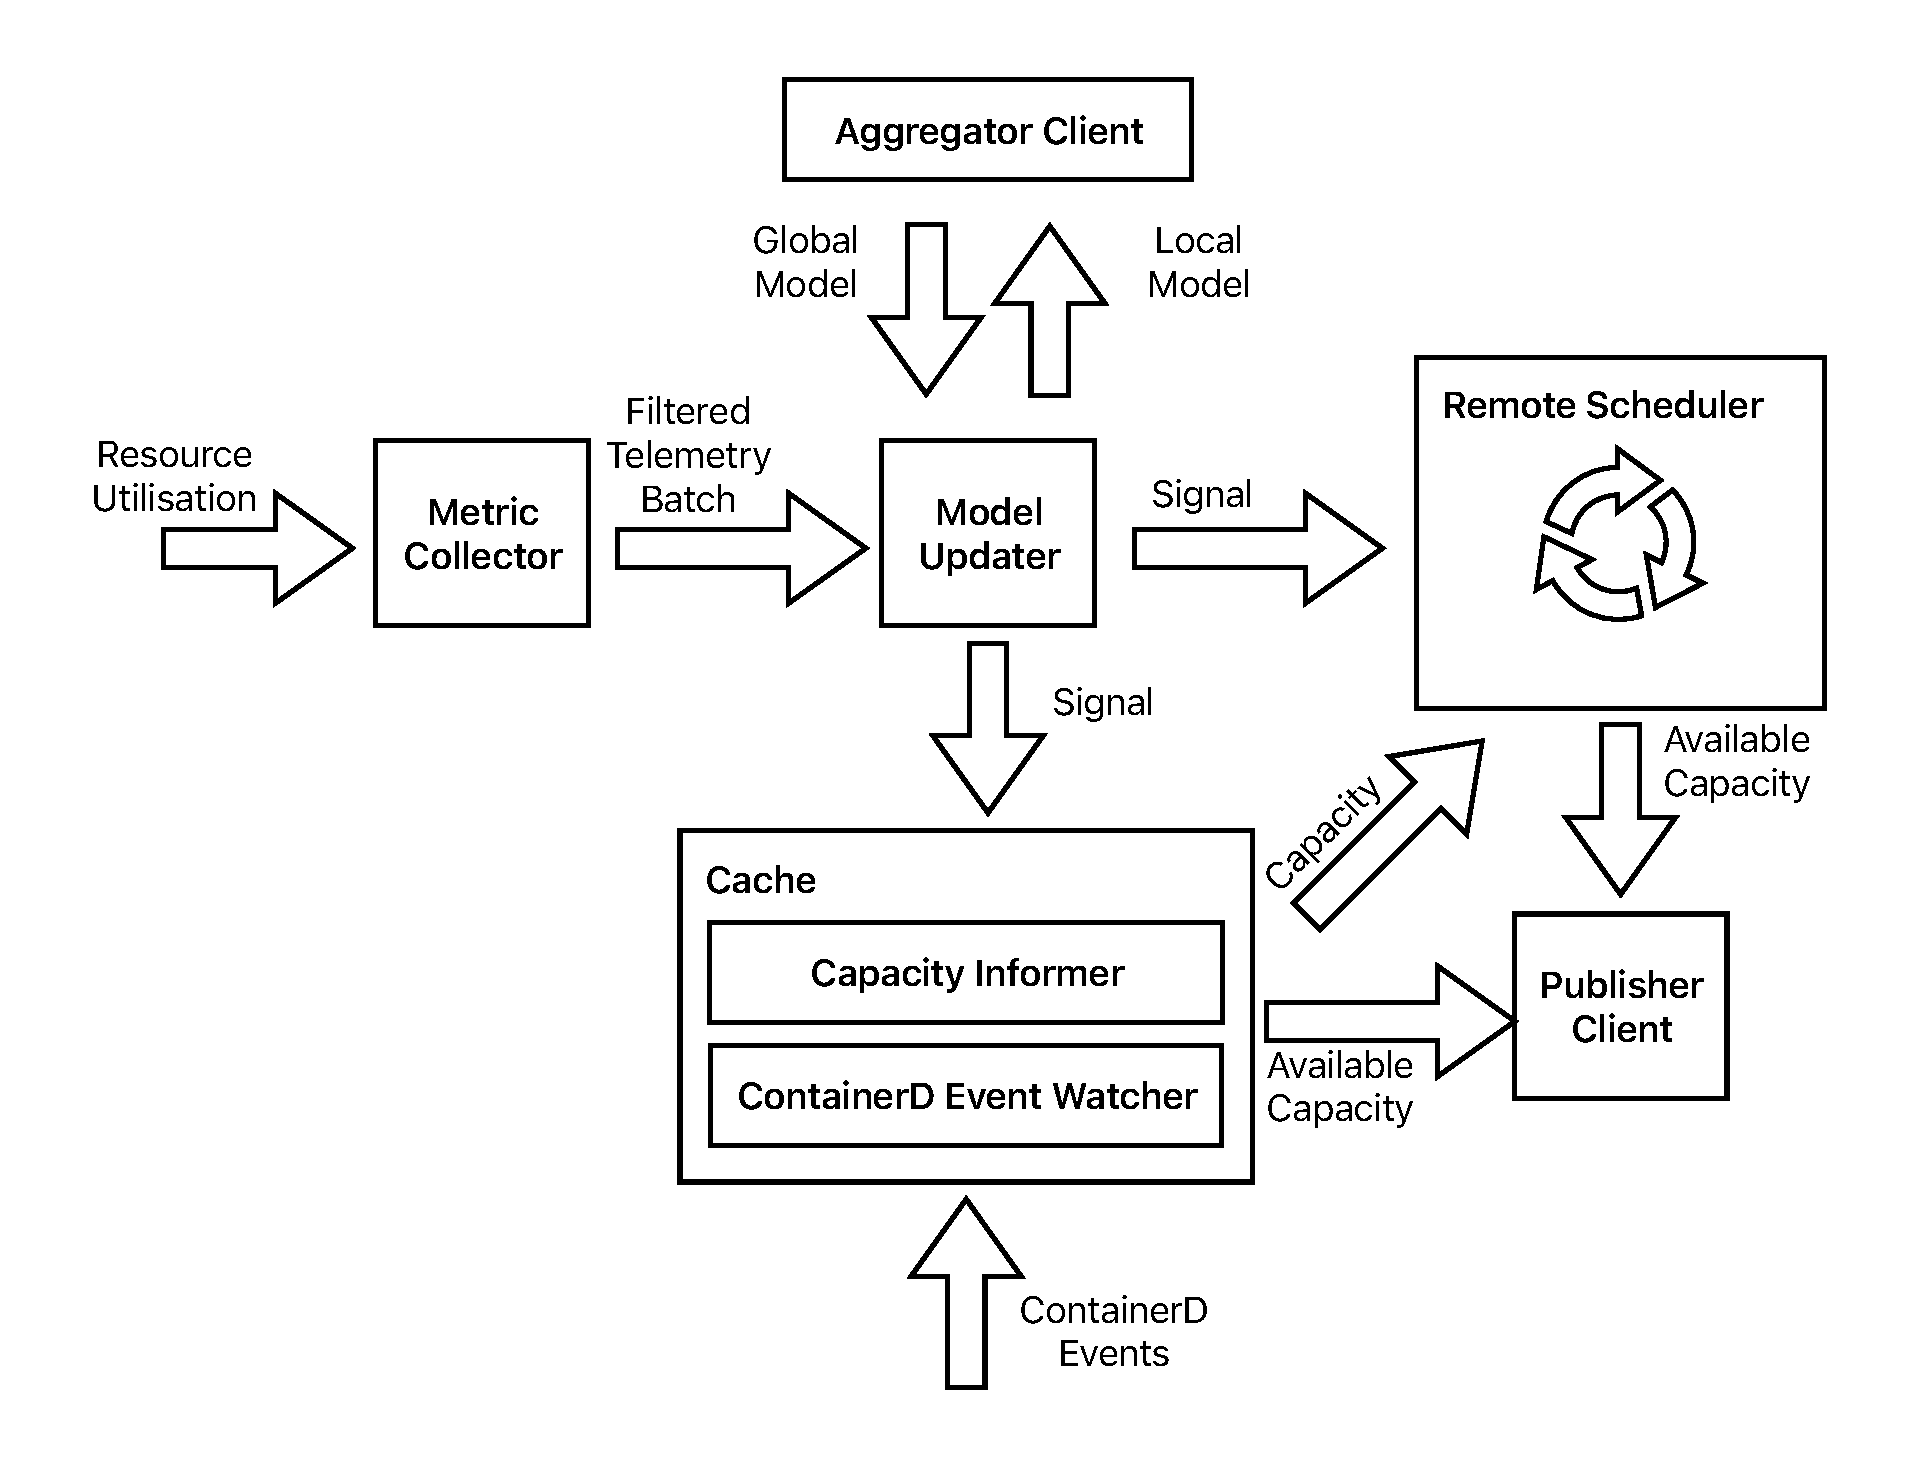
\includegraphics[width=\textwidth]{images/pronto-pod.pdf}
    \caption{Core components within the remote scheduler pod}
    \label{pronto-pod-components}
\end{figure}
As mentioned in section \ref{sec:sys-arch}, the signals are generated by pods
defined by a DaemonSet: each node will contain a single pod which performs the
core functionality of the Pronto system shown in figure
\ref{pronto-pod-components}.

\subsection{Aggregation Component}
\begin{figure}[h]
    \centering
    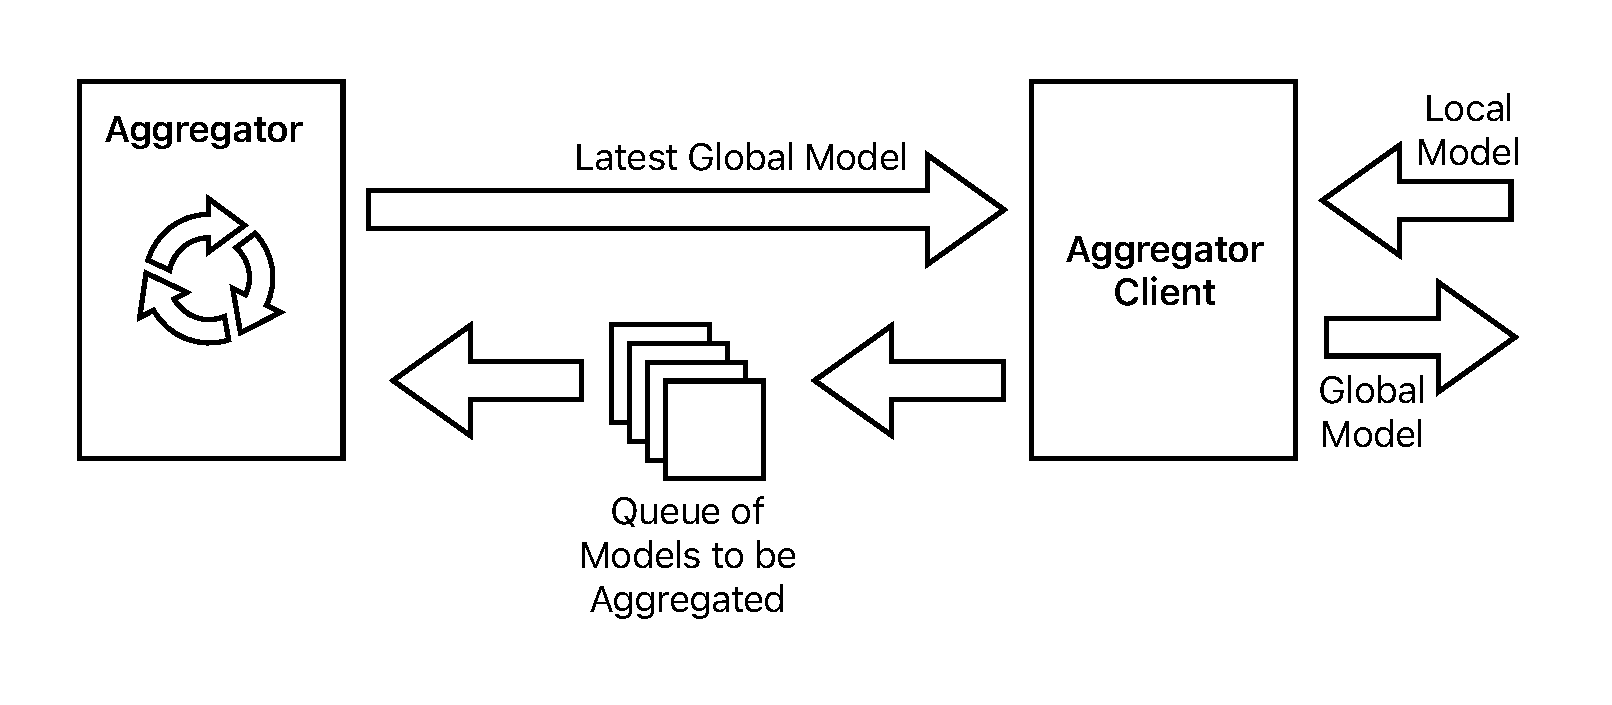
\includegraphics[width=\textwidth]{images/pronto-agg.pdf}
    \caption{Core components within the aggregator pod}
    \label{pronto-agg-components}
\end{figure}

As mentioned earlier in section \ref{sec:aggregation}, the aggregator trades
consistency for latency and throughput. On aggregation request it returns the
latest global model and enqueues the local model it received. Another worker
thread running in the background dequeues local models and merges them into the
global model.

\subsection{Scheduler Component}
\begin{figure}[h]
    \centering
    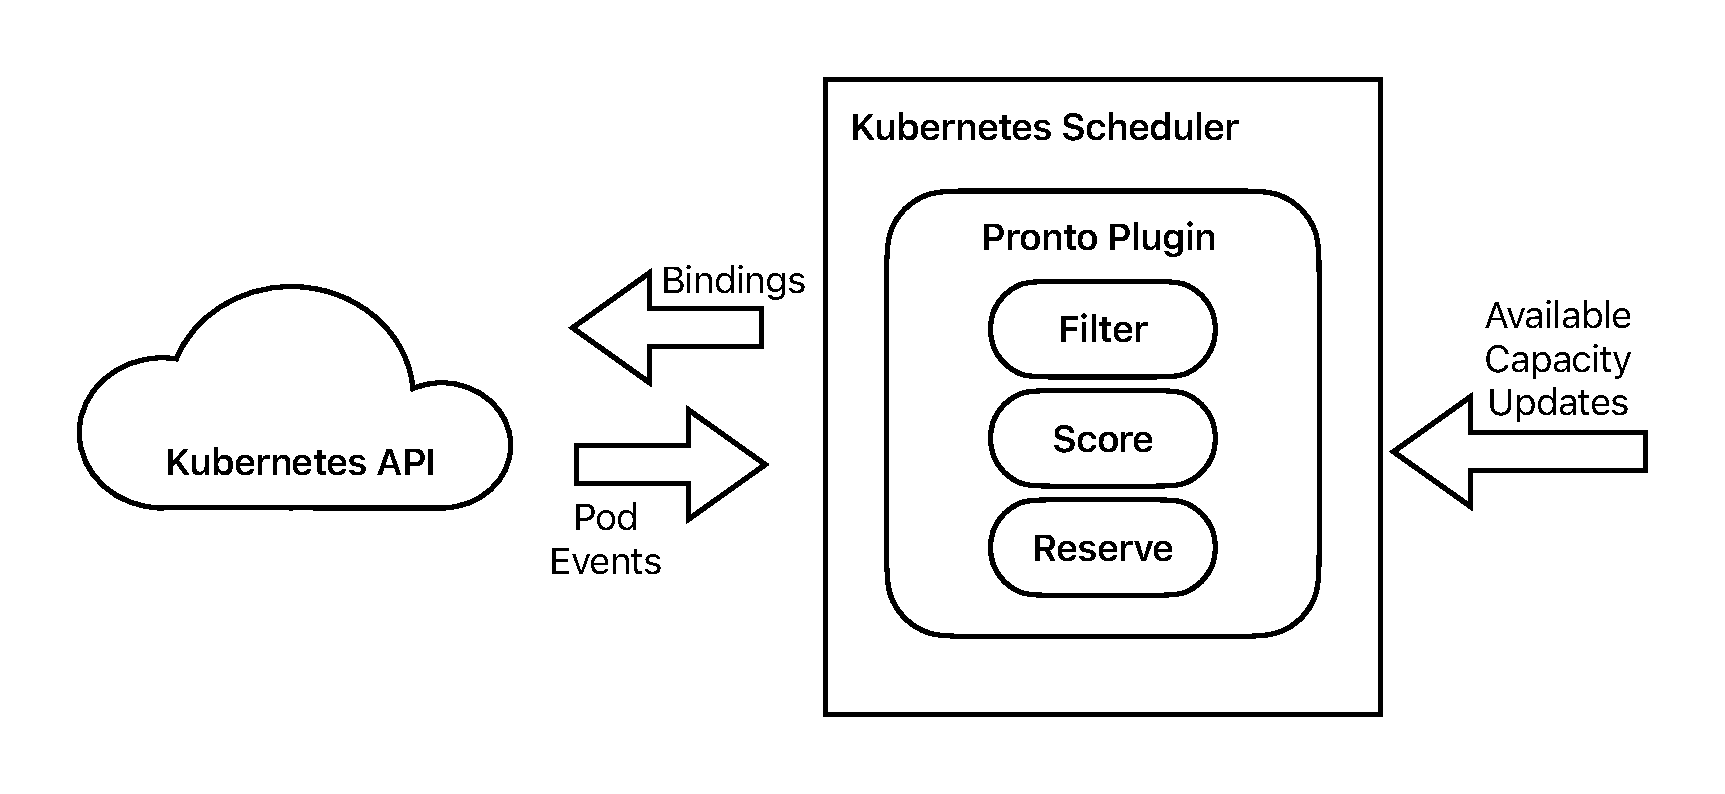
\includegraphics[width=\textwidth]{images/pronto-sched.pdf}
    \caption{Core components within the central scheduler pod}
    \label{pronto-agg-components}
\end{figure}

I decided to implement the scheduling component as a Kubernetes Framework
Plugin. The standard Kubernetes scheduler exposes a series of extension points,
which allows users to define custom functions within the scheduling cycle. A
Scheduler Plugin is a more favourable approach as it allows me to use an
existing system designed to operate at an industrial level. The Pronto Plugin
implements the following extension points:
\begin{itemize}
    \item: Filter - this function filters out any nodes based on $
        \text{capacity available} - \text{capacity reserved} < \epsilon$.
    \item Score - this function assigns a score based on the available capacity.
        The greater the available capacity, the greater the score and thus the
        more likely it is to be chosen for pod placement
    \item Reserve - once a node is chosen to host the pod, the reserve function
        records the pod's name and increments the node's reserved capacity.
\end{itemize}

This pod also has a Kubernetes API Pod Event listener which listens out for pods
that have transitioned from the Pending status. For each event that this occurs,
it checks if this pod was scheduled by the scheduler and decrements its value
from reserved.

\section{Throughput and Optimisations}

\subsection{Observed Sub-Linear Latency Scaling}
While evaluating the prototype, I was stumped by its lackluster throughput
compared to \verb|kube-scheduler|. When deploying 1000 pods across 19 nodes,
\verb|kube-scheduler| would immediately distribute all pods fairly across all
the nodes. This resulted in $\approx$ 45 pods running on each node. Whereas, the
Pronto prototype ensured that no resource was fully utilised and had at most 5
pods running on a node at once. While the individual pod completion time was far
lower, it resulted in a lower throughput.

\begin{figure}[h]
    \centering
    
\includegraphics[width=\textwidth]{images/blank.pdf}
    \caption{Pod completion time against the number of pods running on a node at
    once.}
    \label{fig:number-vs-completion}
\end{figure}

Further investigation in the relationship between the number of pods running on
a node at a time and their completion time showed a sub-linear relationship;
shown in figure \ref{fig:number-vs-completion}. I hypothesise that this is
caused by CPU utilisation not being a representative utilisation metric. While a
node may reach 100\% CPU utilisation, it means that a CPU is always doing work,
but it does not guarantee threads are experiencing high contention. Therefore,
CPU utilisation is not a definitive measure of resource capacity, and explains
why the prototype is not able to push through in terms of pod count and achieve
higher throughput.

\subsection{TCP-style Optimisation}
The goal of the optimisation is to artificially increase the capacity of the
node, as long as it does not push pod completion time beyong a limit and
deteriorate QoS. An additional requirement is that the method needs to be as
efficient as possible while also being able to handle pods of different
workloads and completion times without the requirement of pod-descriptions.


\begin{figure}[h]
    \centering
    
\includegraphics[width=\textwidth]{images/blank.pdf}
    \caption{Example trace of this over-provision capacity exhibiting TCP
    Saw-tooth trend.}
    \label{fig:overprovision-sawtooth}
\end{figure}

To achieve this, I decided to borrow the concept from TCP flow-control. This
method uses a moving window of the latest n pod completion times, with the goal
to identify deteriorating QoS. When receiving a new pod completion time, I
update in O(1) time $\sum (\text{completion time})^2$. By squaring the
completion times, the sum penalizes more longer pod completions that have
increased. It then checks if the new sum is less than the threshold (previous
sum scaled by a constant). If below, we can increment the over-provision
capacity. However, if the new sum exceeds the threshold, the over-provision
capacity is halved. This results in a similar saw-tooth behaviour as seen in TCP
transmissions and allows the node to artificially increase capacity while
mitigating increases in completion times.

